\documentclass[tikz, border = 1 cm]{standalone}

%%%%%%%%%%%%%%
\usepackage{bm}
\usepackage{tikz}
\usetikzlibrary{decorations}
\usetikzlibrary{decorations.markings}	
%%%%%%%%%%%%%%

%%%%%%%%%%%%%%
\definecolor{bluegray1}{RGB}{0,127,167}
\definecolor{orange1}{RGB}{255,126,46}
\definecolor{gray3}	{RGB}{165,169,174}	
\def\opac{0.3}
\def\opacc{0.5}
%%%%%%%%%%%%%%

%%%%%%%%%%%%%%
%%%%%%%%%%%%%%
%%%%%%%%%%%%%%
\begin{document}

%%%%%%%%%%%%%%
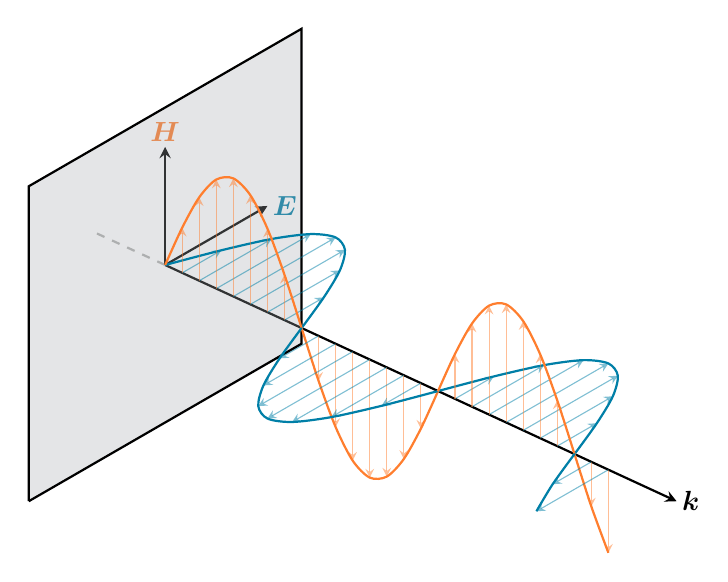
\begin{tikzpicture}[	x={(0.866cm,-0.4cm)}, y={(0.866cm,0.5cm)}, z={(0cm,1cm)},
				scale=1.0, >=stealth, inner sep=0pt, outer sep=2pt,
				axis/.style={thick,->}, wave/.style={thick,color=#1,smooth},
				polaroid/.style={draw=black,thick,fill=gray3,fill opacity=\opac}]

	\def\size{2.0}

	% Frame
	\coordinate (O) at (0,0,0);
	\draw[axis] (O) -- +(7.5,0,0) node [right] {$\bm{k}$};
	\draw[axis] (O) -- +(0,0.75*\size,0) node [right,color=bluegray1] {$\bm{E}$};
	\draw[axis] (O) -- +(0,0,0.75*\size) node [above,,color=orange1] {$\bm{H}$};
	\draw[thick,dashed,opacity=\opac] (-1,0,0) -- (O);
	\filldraw[polaroid] (0,-\size,-\size) -- (0,-\size,\size) -- (0,\size,\size) -- (0,\size,-\size) -- (0,-\size,-\size);%

    % Electric field vectors
    \draw[wave=bluegray1, variable=\x,samples at={0,0.25,...,2}] plot (\x,{1.5*sin(0.5*3.14*\x r)},0);
    \foreach \x in{0.25, 0.5, ...,1.75}
    	\draw[color=bluegray1,->,opacity=\opacc] (\x,0,0) -- (\x,{1.5*sin(0.5*3.14*\x r)},0);
    
    % Magnetic field vectors
    \draw[wave=orange1, variable=\x,samples at={0,0.25,...,2}] plot (\x,0,{1.5*sin(0.5*3.14*\x r)});
    \foreach \x in{0.25, 0.5, ...,1.75}
    	\draw[color=orange1,->,opacity=\opacc] (\x,0,0) -- (\x,0,{1.5*sin(0.5*3.14*\x r)});
	
    % Magnetic field vectors
    \draw[wave=orange1, variable=\x,samples at={2,2.25,...,4}] plot (\x,0,{1.5*sin(0.5*3.14*\x r)});
    \foreach \x in{2.25, 2.5, ...,3.75}
    	\draw[color=orange1,->,opacity=\opacc] (\x,0,0) -- (\x,0,{1.5*sin(0.5*3.14*\x r)});
	
    % Electric field vectors
    \draw[wave=bluegray1, variable=\x,samples at={2,2.25,...,4}] plot (\x,{1.5*sin(0.5*3.14*\x r)},0);
    \foreach \x in{2.25, 2.5, ...,3.75}
    	\draw[color=bluegray1,->,opacity=\opacc] (\x,0,0) -- (\x,{1.5*sin(0.5*3.14*\x r)},0);
	
    % Electric field vectors
    \draw[wave=bluegray1, variable=\x,samples at={4,4.25,...,6}] plot (\x,{1.5*sin(0.5*3.14*\x r)},0);
    \foreach \x in{4.25, 4.5, ...,5.75}
    	\draw[color=bluegray1,->,opacity=\opacc] (\x,0,0) -- (\x,{1.5*sin(0.5*3.14*\x r)},0);
	
    % Magnetic field vectors
    \draw[wave=orange1, variable=\x,samples at={4,4.25,...,6}] plot (\x,0,{1.5*sin(0.5*3.14*\x r)});
    \foreach \x in{4.25, 4.5, ...,5.75}
    	\draw[color=orange1,->,opacity=\opacc] (\x,0,0) -- (\x,0,{1.5*sin(0.5*3.14*\x r)});
	
    % Magnetic field vectors
    \draw[wave=orange1, variable=\x,samples at={6,6.25,...,6.5}] plot (\x,0,{1.5*sin(0.5*3.14*\x r)});
    \foreach \x in{6.25, 6.5}
    	\draw[color=orange1,->,opacity=\opacc] (\x,0,0) -- (\x,0,{1.5*sin(0.5*3.14*\x r)});
	
    % Electric field vectors
    \draw[wave=bluegray1, variable=\x,samples at={6,6.25,...,6.5}] plot (\x,{1.5*sin(0.5*3.14*\x r)},0);
    \foreach \x in{6.25, 6.5}
    	\draw[color=bluegray1,->,opacity=\opacc] (\x,0,0) -- (\x,{1.5*sin(0.5*3.14*\x r)},0);
	    
\end{tikzpicture}
%%%%%%%%%%%%%%

\end{document}